\documentclass[12pt,a4paper]{report}
\usepackage{amssymb,amsthm,amsmath,amscd}
\usepackage{latexsym}
\usepackage{enumerate}
\usepackage[german]{babel}
\usepackage{verbatim}
\usepackage[hyphens]{url}
\usepackage{hyperref}
\usepackage[utf8]{inputenc}
\usepackage{pdfpages} 
\usepackage{graphicx}

\begin{document}
\begin{titlepage}
	\begin{center}
		
		\vspace*{1.0cm}
		\huge
		\textsc{\bf{PS Algorithmen für verteilte Systeme}}
		
		\vspace*{4.0cm}
		\textsc{
			\normalsize{eingereicht von} \\[0.5\baselineskip]
			{\large Baumgartner Dominik, Dafir Samy}
		}
		
		\vspace*{3.0cm}
		\textsc{
			\normalsize{Gruppe  1(16:00)}
		}
		
	\end{center}
	
\end{titlepage}
\ \\
\textbf{Aufgabe 6:}
Zeigen Sie, dass $CCC(k)$ Teilgraph des $BF(k)$ ist.
\\
Z.z.: Für jedes n  $\in \mathbb{N}$ gilt: $CCC(n)$ ist ein Teilgraph von $BF(n)$.\\
\\
Bew.:\\
Sei Sei n  $\in  \mathbb{N}$. Definieren folgende Funktion:
\begin{center}
$p$ : $V \rightarrow V$ $|$ $p((i,$ $b)):=((i + k(b))mod(n),$ $b)$.
\end{center}
wobei $i$ das aktuelle Level ist und b ein Bitfolge der Länge n. Zudem gilt:\\
$k(b) := \begin{cases}\text{1, wenn b ungerade Anzahl an 1er Bits besitzt}\\\text{0, sonst}\end{cases}$
\\
\\
Wird nun die Funktion $v$ auf den $CCC(n)$ angewendet, werden alle Knoten von $CCC(n)$ auf $BF(n)$ abgebildet. Anhand der folgenden Abbildung ist zu erkennen, dass die Funktion $v$ auch bijektiv ist.
\begin{center}
	\includegraphics{ccc-zu-bf.png}
\end{center}
\ \\
Noch zu zeigen, dass auch jede Kante von $CCC(n)$ auf eine Kante von $BF(n)$ abgebildet wird:\\
$\forall e$ = $\{u,v\}$  $\in$ $E_{CCC}$ gilt $p(e)$ := $\{p(u),p(v)\}$  $\in$ $E_{BF}$.\\
\newpage
\ \\
Für jedes $e$ $\in$ $E_{CCC}$ gibt es zwei Fälle:\\
1. Fall:\\
$x$ = $\{(i,$ $b),$ $((i + 1)mod(n),$ $b)\}$ $\in$ $E_{C}$. Falls $k(w)$ = 0 ist, so ist $p(x)$ = $x$ und anderenfalls ist 
$p(x)$ = $\{((i + 1)$ $mod$(n)$,$ $b)$, $((i + 2)$ $mod(n),$ $b)\}$ . In beiden Fällen gehört $p(x)$ zu $E_{C}$.\\
2. Fall: \\
$x$ = $\{(i, b), (i, b(i))\}$ $\in$ $E_H$, wobei $b(i)$ die Bitfolge $b$ mit geflippten Bit an Stelle $i$ ist. Falls $k(w)$ = 0 gilt, so ist $k(w(i))$ = 1 und \\
$p(x)$ = $\{(i, b), ((i + 1)$ $mod(n)$, $b(i))\}$. \\
Sonst ist $p(x)$=$\{((i + 1)$ $mod(n),$ $b),$ $(i,$ $b(i))\}$. In beiden Fällen ist $p(x)\in E_X$. \\
\newpage
\textbf{Aufgabe 7:}
Zeigen Sie, dass das Butterfly-Netzwerk $BF(k)$ knotensymmetrisch ist.
\\
\begin{figure}[!hb]
	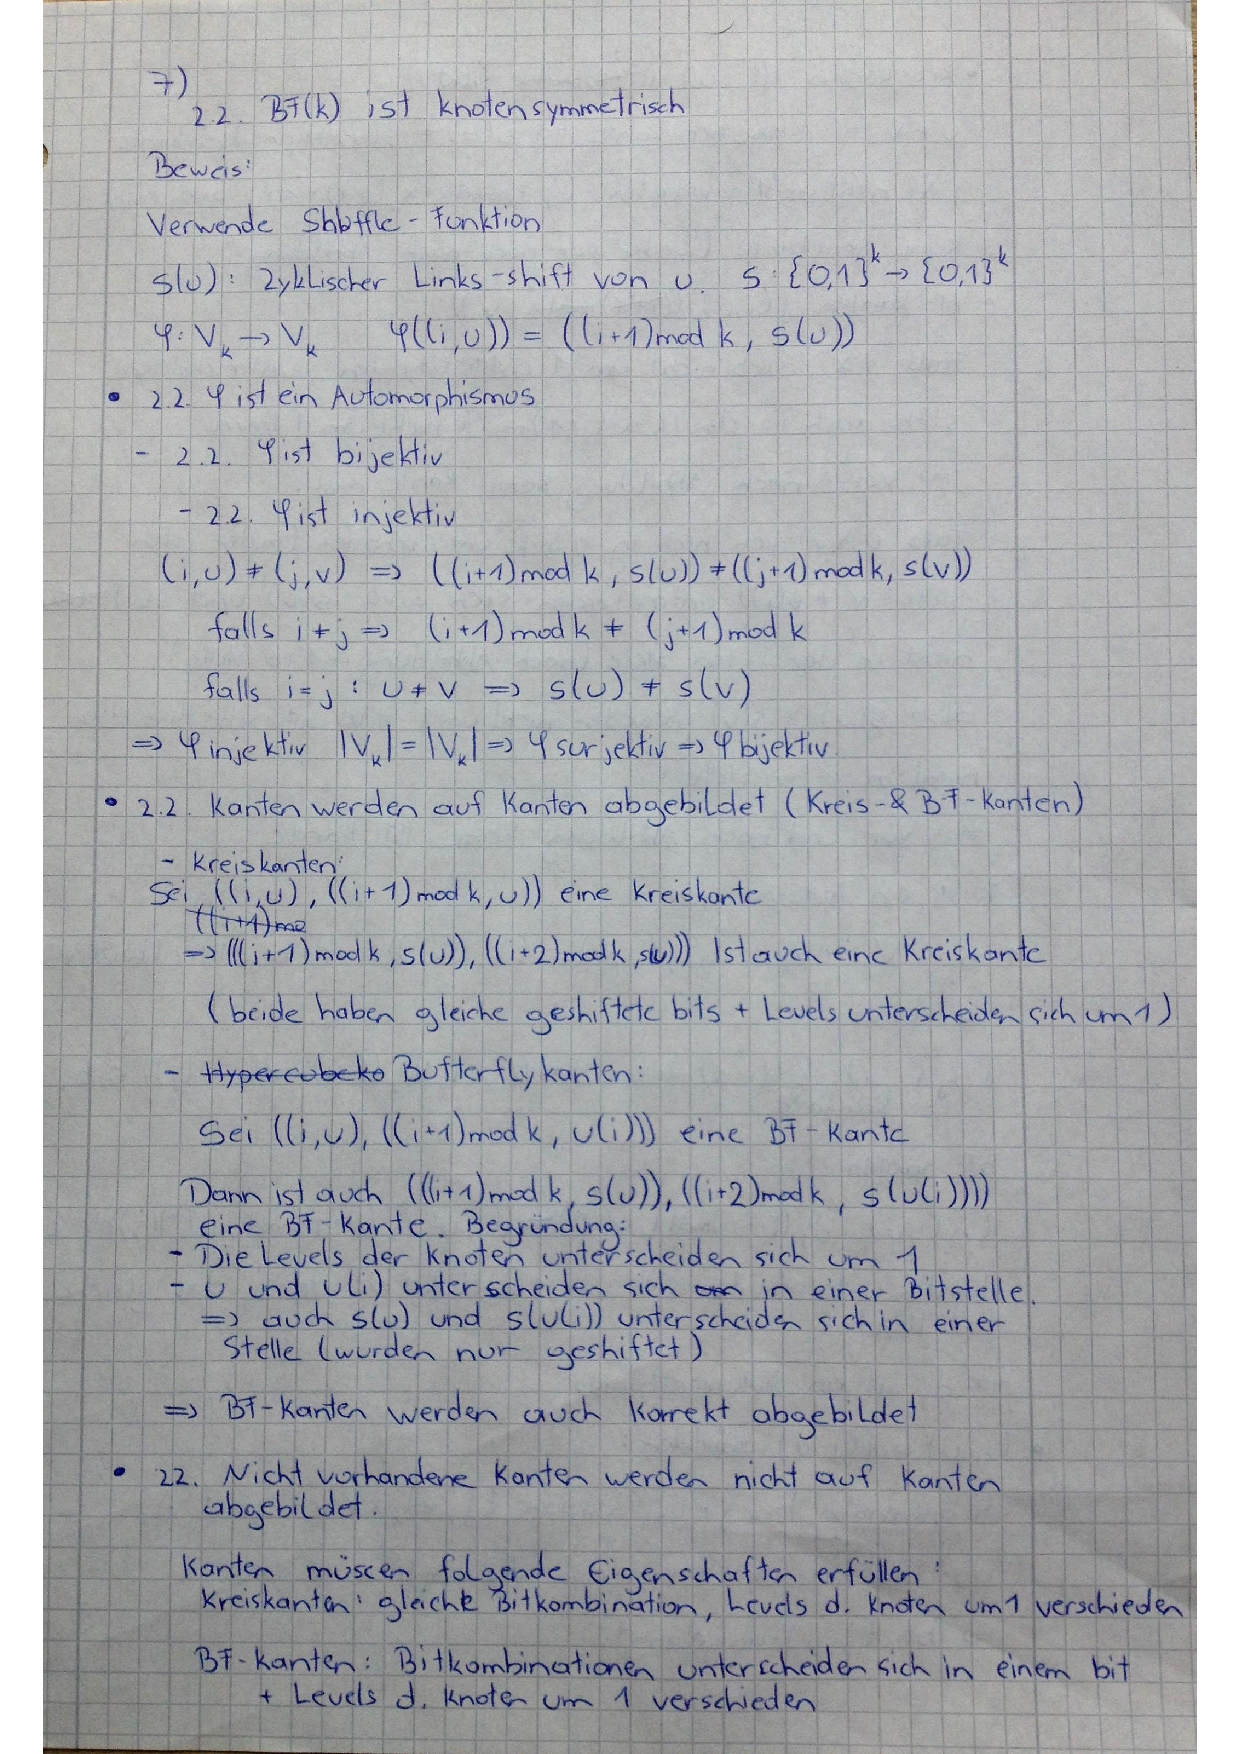
\includepdf[height=18cm, width=16cm]{7.pdf}
\end{figure}
\includepdf[height=18cm, width=16cm]{7-2.pdf}

\textbf{Aufgabe 5:}
Schreiben Sie ein Programm, dass das folgende Viceroy-Netzwerk
erstellt. Weisen Sie zunächst 100 Knoten 5 Ringen zu, wie in der Vorlesung
beschrieben. Erstellen Sie anschließend die in der Vorlesung definierten
Verbindungen zwischen diesen Knoten. Wählen Sie 100 Knotenpaare
zufällig aus und berechnen Sie Routing-Pfade zwischen diesen Knotenpaaren.
Bei der Berechnung eines Routing-Pfades dürfen Sie ausschließlich auf
lokale Nachbarschaftsinformationen zurückgreifen. Geben Sie anschließend
die Verteilung der Längen dieser Routing-Pfade aus.
\\
\\
In der folgenden Graphik ist die Verteilung der Längen der Routing-Pfade abgebildet.
\begin{center}
	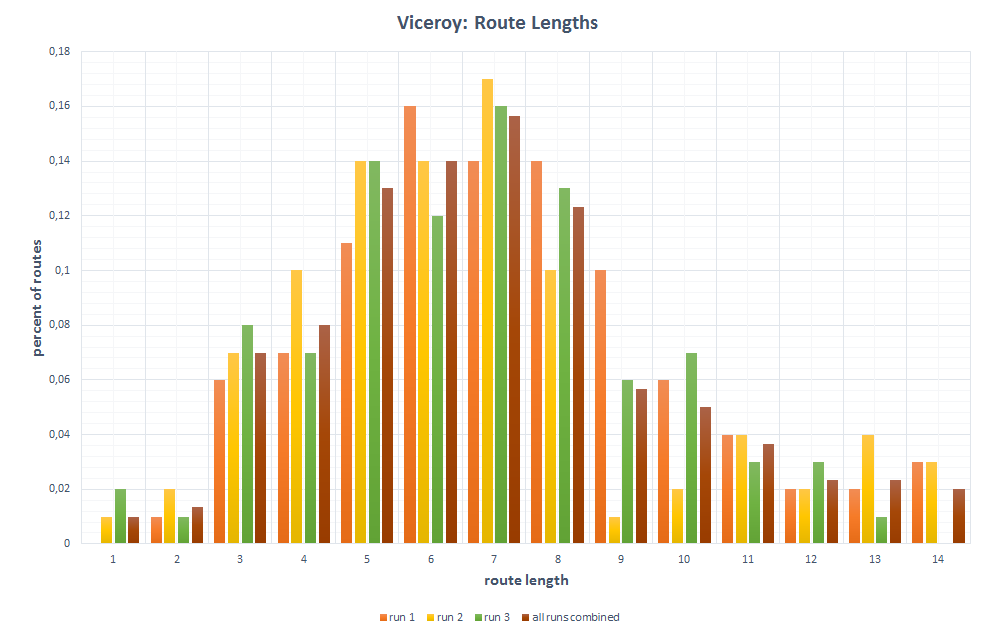
\includegraphics[height=10cm, width=15cm]{auswertung.png}
\end{center}

\end{document}

